\renewcommand{\theauthor}{Dario Wagner}
\justifying
\section{Parser}
\label{sec:parser}
\subsection{Aufgabe}
\label{sec:parser-aufgabe}
Die Aufgabe des Parsers ist es auf die Datenbank zuzugreifen und sich die, für das iCal Format notwendigen, Daten zu holen. Diese werden anschließend vom Parser in einen iCal String umgewandelt, damit der benutzte Kalender diesen verwerten kann und passende Termine erstellt. 

\subsubsection{Source-Code}
%Hier kommt die Erklärung des Source Codes hin

\subsection{Entity Framework}
\label{sec:parser-entity-framework}
\subsubsection {Funktionsweise}
Mithilfe des Entity Framework lässt sich eine Datenbankstruktur innerhalb des Projekts mit Klassen darstellen. Wenn auf eine dieser Klassen in Form einer Value-Abfrage zugegriffen oder durch sonstige GET/SET Methoden, wird durch das Entity Framework ein Datenbank Zugriff durchgeführt. 
Um die Funktionsweise genauer zu verstehen folgt ein Beispiel mit einer Datenbank in welcher Autos gespeichert werden:
HIER KOMMT DANN EIN BEISPIEL
\subsubsection {Anwendung}
Voraussetzung: Funktionsfähige ASP.NET Web Application \\
\break \textbf{1. Erstellung einer Datenbank} \\
Als Beispiel wurde für dieses Beispiel die Scott Tiger Datenbank verwendet.
\break \url{http://jailer.sourceforge.net/scott-tiger.sql.html} \\
\break \textbf{2. Installieren des EntityFrameworks} \\
In der Packet Manager Console folgenden Befehl eingeben und bestätigen: 
\begin{figure}[H]
    \centering
    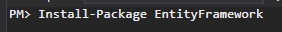
\includegraphics[width=0.5\textwidth]{Parser_EFUse01}
    \caption{Install}
    \label{fig:parsef01}
\end{figure}
Abschluss der Installation sieht wie folgt aus:
\begin{figure}[H]
    \centering
    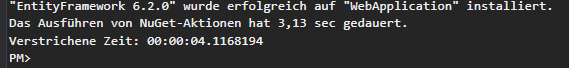
\includegraphics[width=0.9\textwidth]{Parser_EFUse02}
    \caption{Install complete}
    \label{fig:parsef02}
\end{figure} 

\break \textbf{3. Entity Framework generiert Klassen aus DB} \\
Im Solution Explorer auf den Model Ordner Rechtsklick machen -> ''Hinzufügen'' -> ''Neues Element''
\begin{figure}[H]
    \centering
    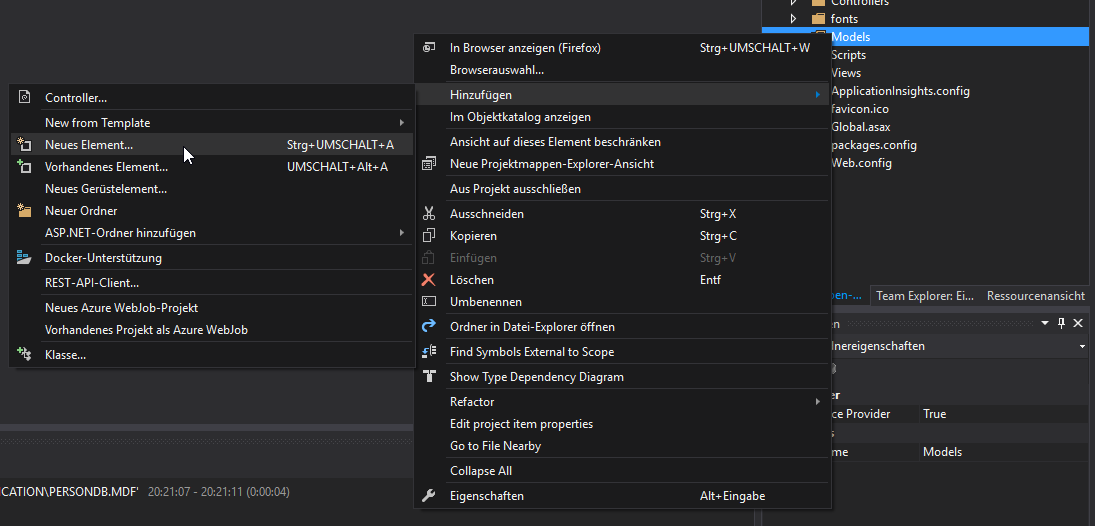
\includegraphics[width=\textwidth]{Parser_EFUse03}
    \caption{Neues Element}
    \label{fig:parsef03}
\end{figure} 
Anschließend auf ''Daten'' -> ''ADO.NET Entity Data Model'' -> Hinzufügen
\begin{figure}[H]
    \centering
    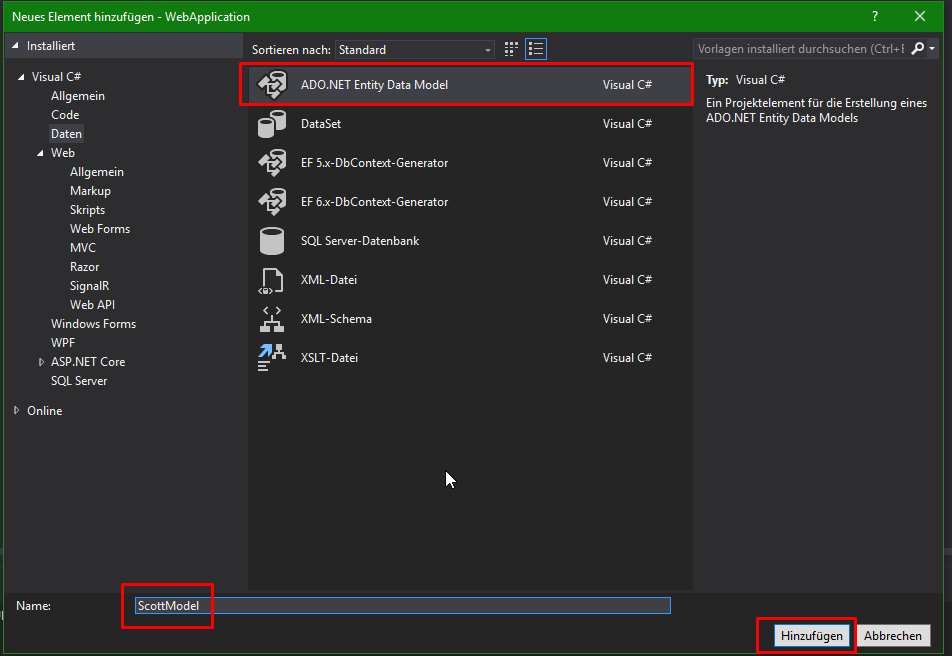
\includegraphics[width=\textwidth]{Parser_EFUse04}
    \caption{ADO.NET Entity Data Model}
    \label{fig:parsef04}
\end{figure} 
Im nächsten Fenster nun  ''EF Designer aus Datenbank'' auswählen und ''Weiter''
\begin{figure}[H]
    \centering
    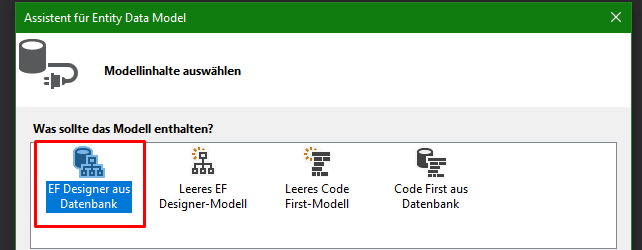
\includegraphics[width=\textwidth]{Parser_EFUse05}
    \caption{EF Designer aus Datenbank}
    \label{fig:parsef05}
\end{figure} 
Hier zunächst die Verbindung auswählen in diesem Fall ist ein lokales Datenbankfile vorhanden, daher wird dieses per DropDownMenü ausgewählt und auf ''Weiter''
\begin{figure}[H]
    \centering
    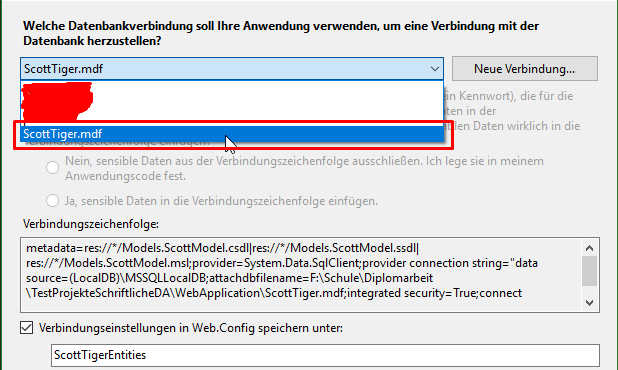
\includegraphics[width=\textwidth]{Parser_EFUse06}
    \caption{Datenverbindung}
    \label{fig:parsef06}
\end{figure} 
Alle Tabellen auswählen und auf ''Fertig stellen''. 
\begin{figure}[H]
    \centering
    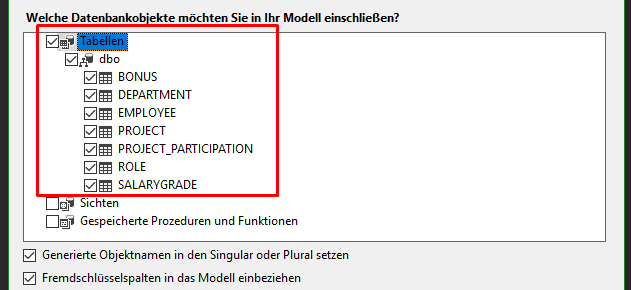
\includegraphics[width=\textwidth]{Parser_EFUse07}
    \caption{Datenbankobjekte auswählen}
    \label{fig:parsef07}
\end{figure} 
Falls eine Sicherheitswarnung erscheint auf ''OK'' klicken. \\
Endresultat, das Entity Framework hat die Tables im Models Ordner erstellt und am Bildschirm sieht man das Klassen mit ihren Beziehungen. Dies sollte ungefähr so aussehen:
\begin{figure}[H]
    \centering
    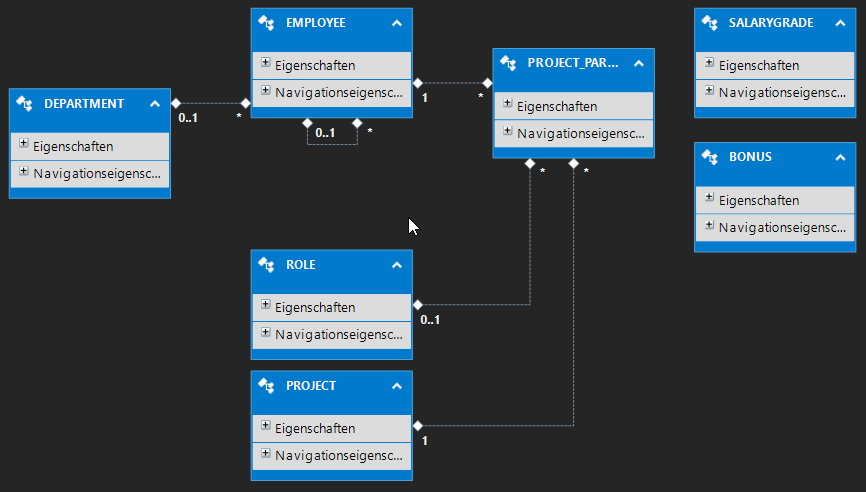
\includegraphics[width=\textwidth]{Parser_EFUse09}
    \caption{Klassendiagramm}
    \label{fig:parsef07}
\end{figure} 
\begin{figure}[H]
    \centering
    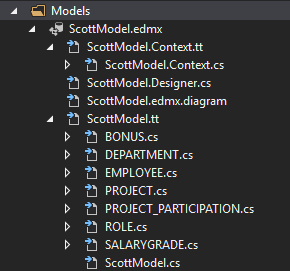
\includegraphics[width=0.5\textwidth]{Parser_EFUse10}
    \caption{Solutionsexplorer}
    \label{fig:parsef07}
\end{figure} 



\subsubsection{Source-Code}
%Hier kommt die Source-Code Erklärung des Parsers hin